\documentclass[pscyr,nonums]{hedlab}
\usepackage[russian]{babel}
\usepackage[utf8]{inputenc}
\usepackage{graphicx}
\usepackage{listings}

\labnum{1}
\labname{Введение в разработку Android-приложений.}
\student{Чечеткин И. А.}
\labdate{}

\begin{document}
  \makeheader
  \lstset{language=java, basicstyle=\tiny}

  \emph{Цель работы:} 
  \begin{enumerate}
    \item познакомится с инструментами разработки Android-приложения,
    \item разобрать структуру типичного Android-приложения,
    \item научиться запускать приложение на эмуляторе,
    \item научиться тестировать приложение с помощью
      Dalvik Debug Monitor Server (DDMS).
  \end{enumerate}

  \vspace{2em}
%  \emph{Приложение:}
  \lstinputlisting{code/calc/src/com/example/calc/MainActivity.java}

  \begin{figure}[!ht]
    \center
    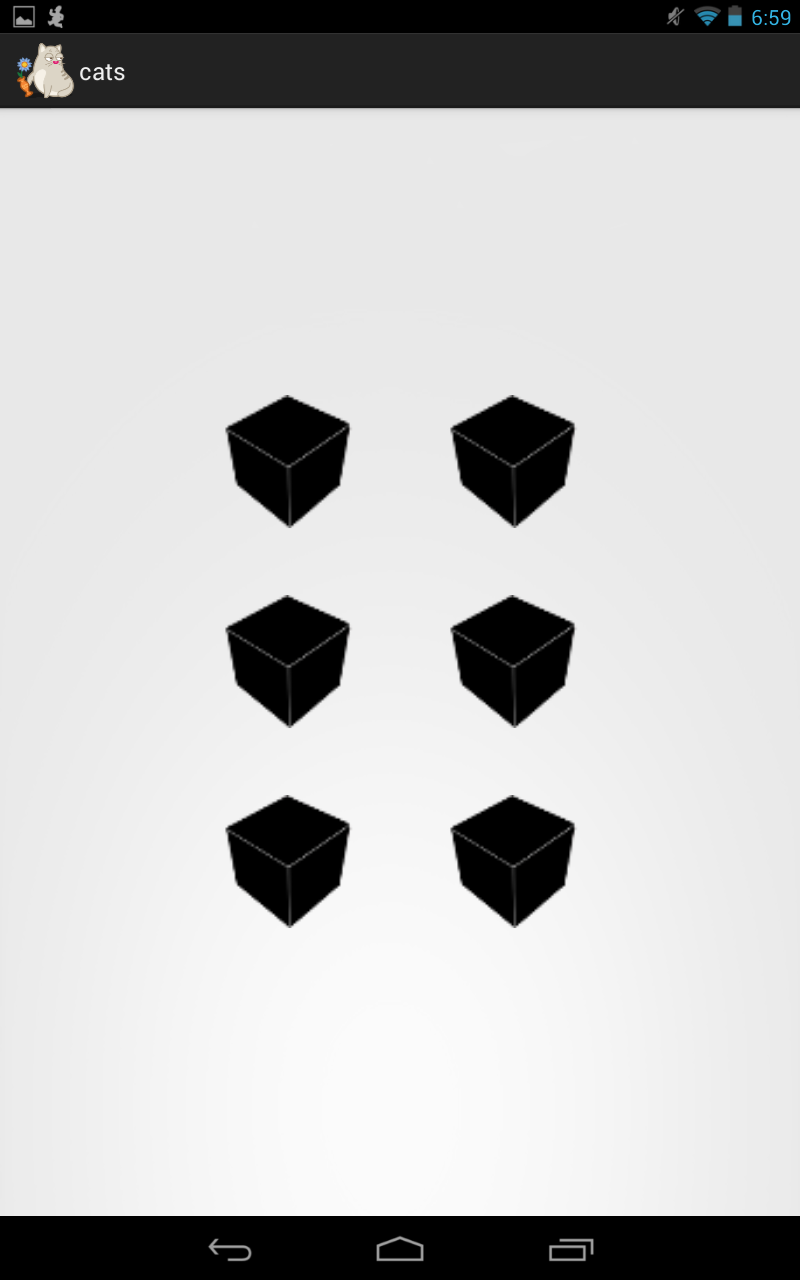
\includegraphics[width=.47\textwidth]{01} \hfill
    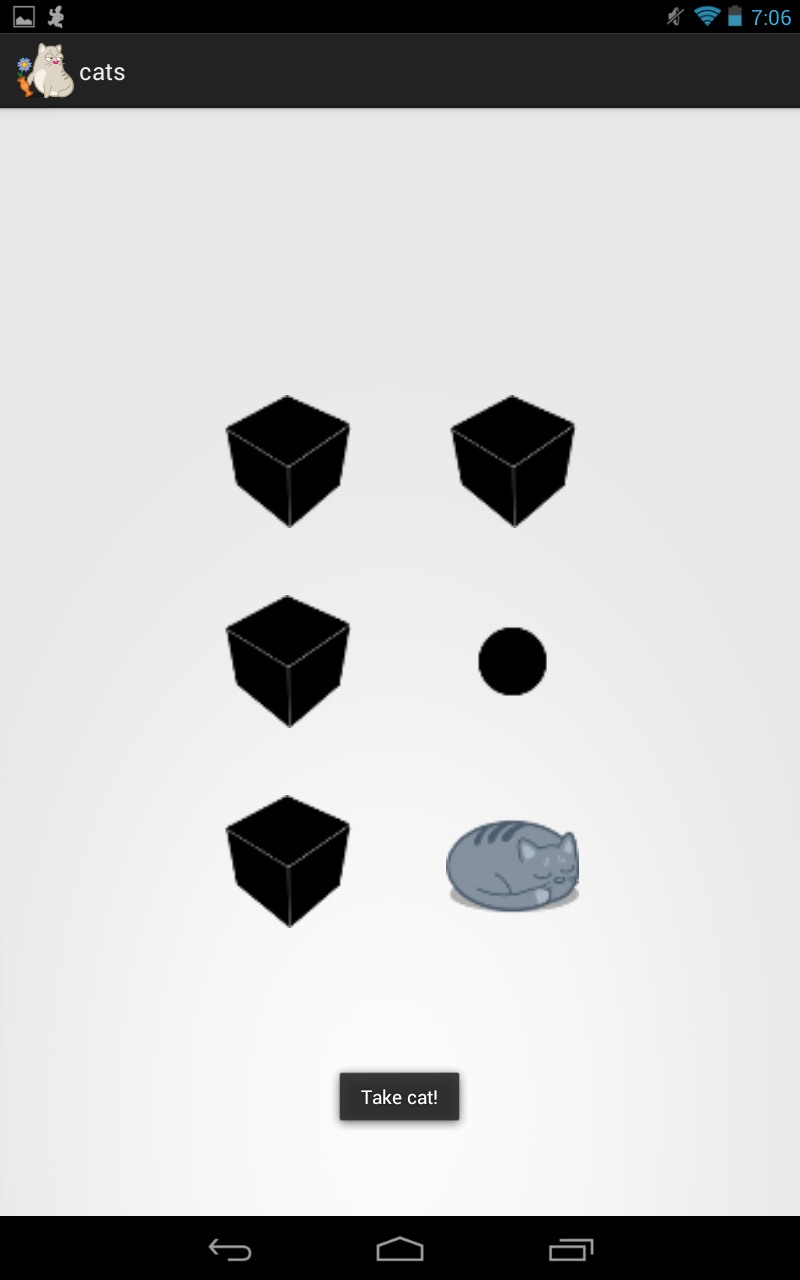
\includegraphics[width=.47\textwidth]{02}
    \caption{Скриншоты приложения}
  \end{figure}
\end{document}
